\documentclass[sigconf, nonacm, timestamp, balance=false,manuscript]{acmart}

\usepackage{ctex}

\usepackage{geometry}
\geometry{a4paper, scale=0.8}

\usepackage{minted}
\setminted{breaklines, breakanywhere, linenos}

\usepackage{relsize}

\usepackage{graphicx}

\usepackage{oz}

\makeatletter
\let\ACM@origbaselinestretch\baselinestretch
\makeatother

\setminted[cpp]
{
    style=xcode,
    mathescape,
    linenos,
    autogobble,
    tabsize=4,
    fontsize=\normalsize,
    %bgcolor=Gray,
    numbersep=1mm,
    breaklines=true,
    breaksymbolsepleft=2pt,
    %breaksymbolleft=\raisebox{0.8ex}{ \small\reflectbox{\carriagereturn}}, %not moe!
    %breaksymbolright=\small\carriagereturn,
    breakbytoken=false,
    showtabs=true,
    tab={\relscale{0.6} $\big\vert \ \ \ $ \relscale{1}},
}

\usepackage{hyperref}

\usepackage{amsmath}

\title{ICPC 使用例暨军训打发时间解决方案}
\author{earthmessenger \& FatOldEight}
\date{癸卯四月十四}

\begin{document}

\begin{teaserfigure}
    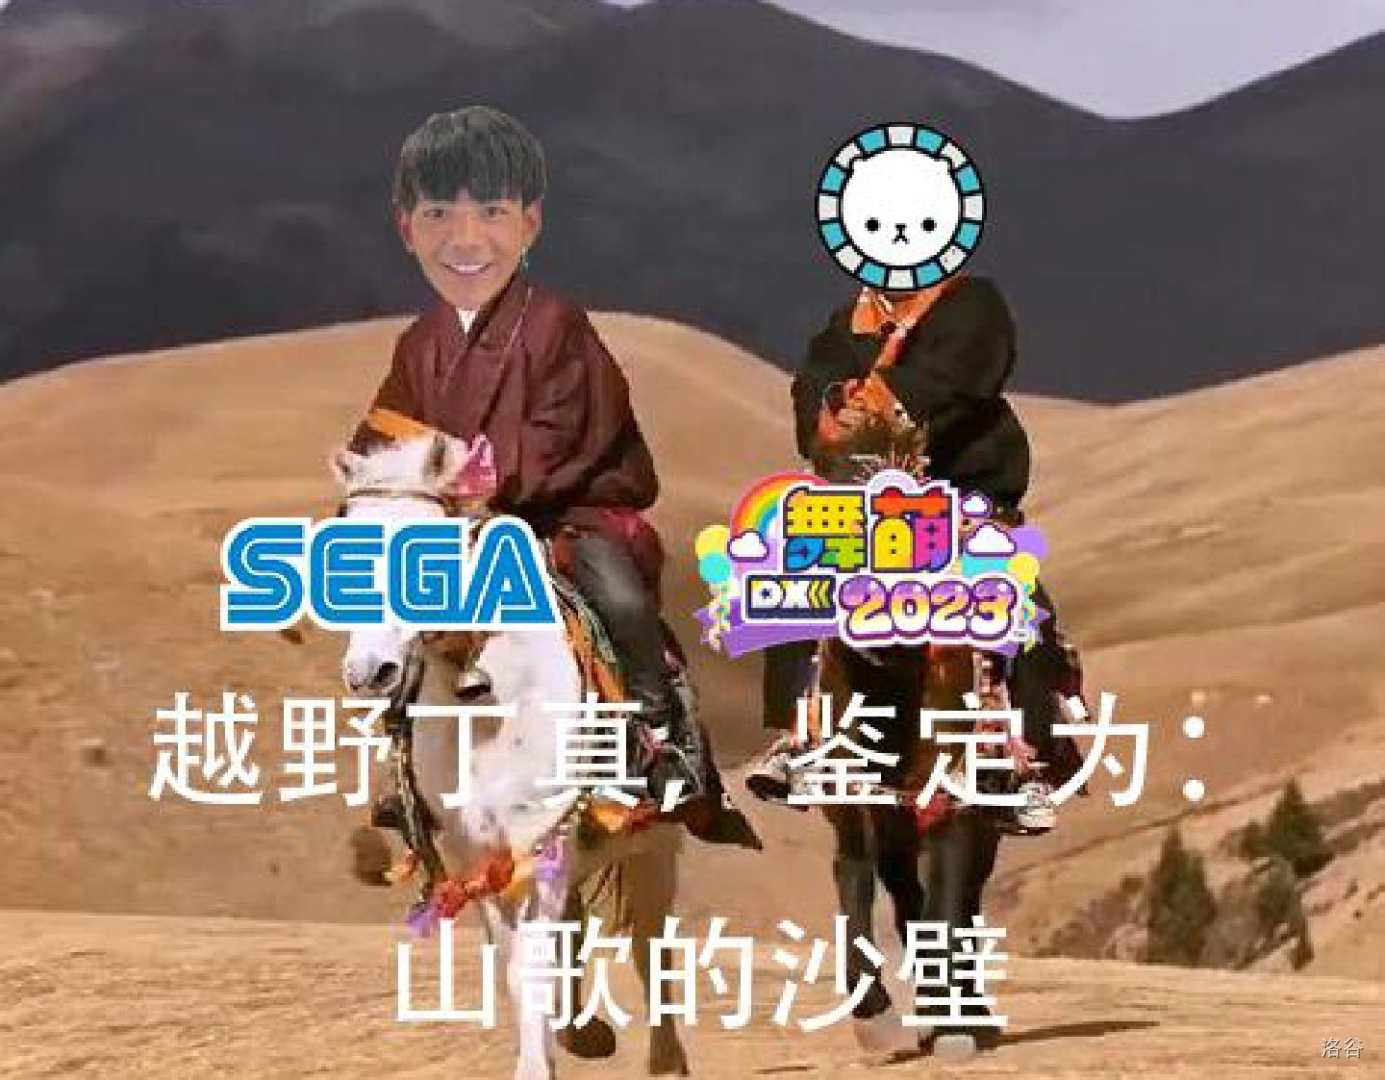
\includegraphics[width=\textwidth]{fa6f4vdw.png}
    \caption{来自甘孜州的选手丁真和iiDX。}
\end{teaserfigure}
\maketitle

% 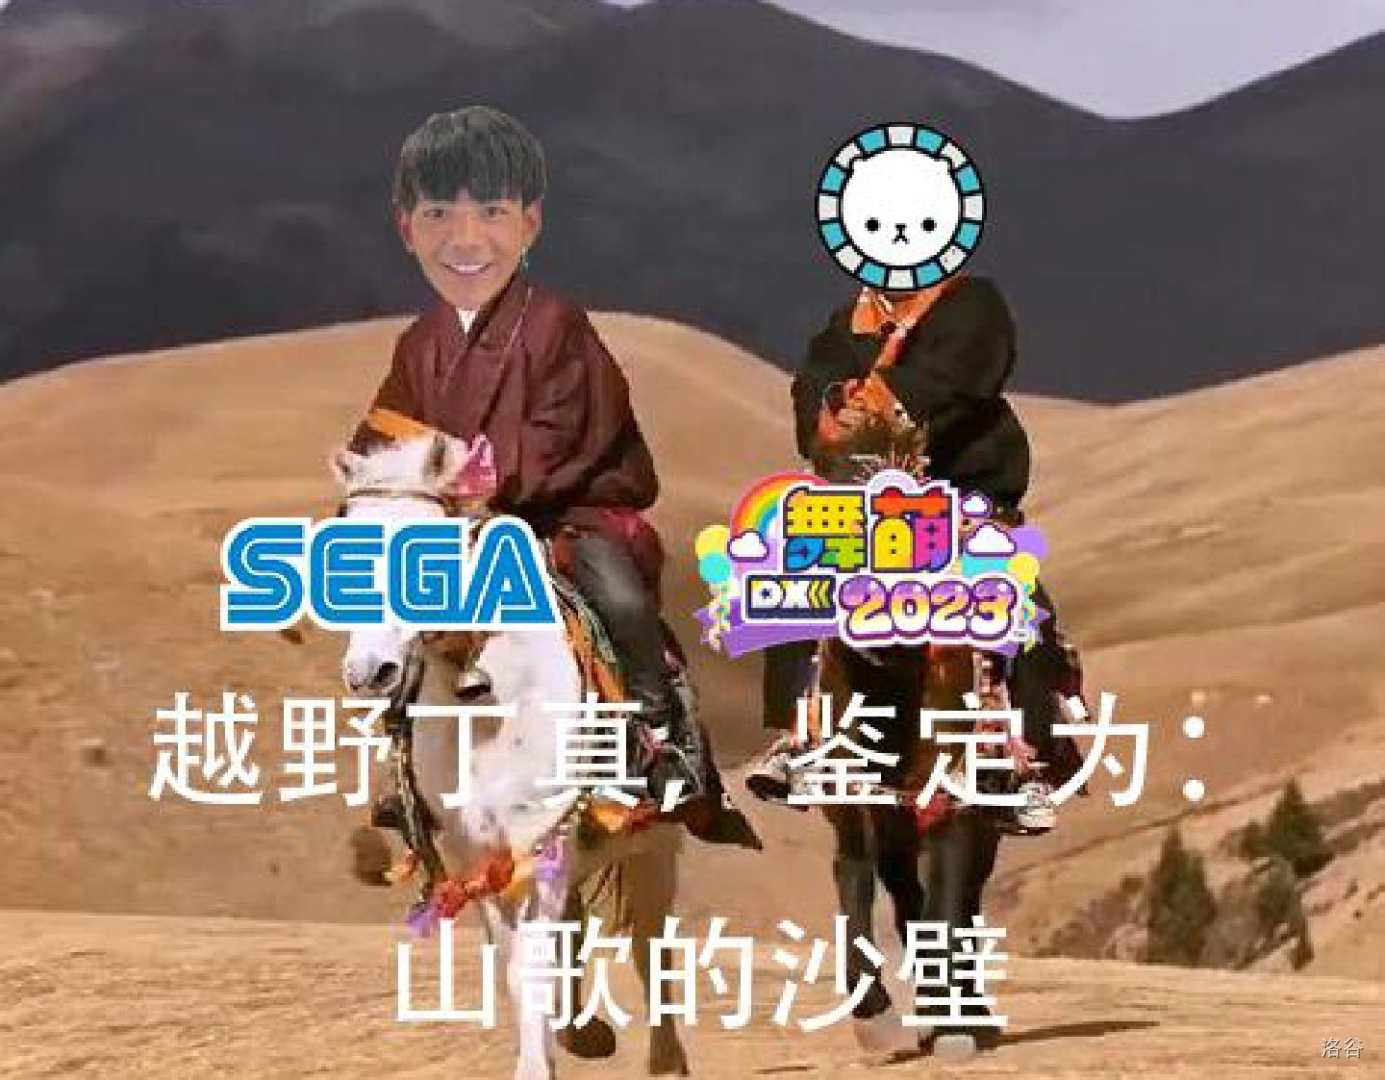
\includegraphics[scale=0.6]{fa6f4vdw.png}

\clearpage

\tableofcontents

\textbf{警告:代码没有经过测试,不能保证其正确性。}

\section{ICPC使用例}

\section{数据结构}

\subsection{FHQ}

仅有分裂和合并。

\inputminted{cpp}{icpc/ds/treap/treap.cpp}

\subsection{李超线段树}

\inputminted{cpp}{icpc/ds/CNM/CNM.cpp}

\section{计算几何}

谢谢 AtCoder。

因为换过模板,所以上面那句话基本作废了。

\subsection{二维计算几何}

\inputminted{cpp}{icpc/geom/geom2d/geom2d.cpp}

\subsection{三维计算几何}

\inputminted{cpp}{icpc/geom/geom3d/geom3d.cpp}

\subsection{平面最近点对}

\inputminted{cpp}{icpc/geom/close/close.cpp}

\subsection{三维凸包}

应该用不上,军训时可以看看。

\inputminted{cpp}{icpc/geom/swtb/swtb.cpp}
\section{图论}

\subsection{Bellman-Ford 算法}

\inputminted{cpp}{icpc/graph/shortest_path/bf.cpp}

\subsection{最大流}

\inputminted{cpp}{icpc/graph/maxflow/maxflow.cpp}

\subsection{费用流}

\inputminted{cpp}{icpc/graph/SSP/SSP.cpp}

\subsection{强连通分量算法}

\inputminted{cpp}{icpc/graph/scc/scc.cpp}

\subsection{树剖}

\inputminted{cpp}{icpc/graph/splittree/splittree.cpp}

\section{数学}

\subsection{线性筛}

欧拉函数不会,所以没写。

\inputminted{cpp}{icpc/math/prime/prime.cpp}

\subsection{高斯消元}

\inputminted{cpp}{icpc/math/gauss/gauss.cpp}

\subsection{乘法逆元}

\subsubsection{线性求逆元}

\inputminted{cpp}{icpc/math/inv/inv.cpp}

\subsubsection{线性求任意 $n$ 个数的逆元}

\inputminted{cpp}{icpc/math/inv/inv_any.cpp}

\subsection{欧几里得算法}

\subsubsection{扩展欧几里得算法}

\inputminted[mathescape]{cpp}{icpc/math/gcd/ex_eculid.cpp}

\subsubsection{高速 gcd}

\[
\gcd\left(a, b\right) = \begin{cases}
\gcd\left[|a - b|, \min(a, b)\right] & \text{a, b 奇} \\
\gcd\left(\frac{a}{2}, \frac{b}{2}\right) & \text{a, b 偶} \\
\gcd\left(a, \frac{b}{2}\right) & \text{a 奇, b 偶} \\
\gcd\left(\frac{a}{2}, b\right) & \text{a 偶, b 奇} 
\end{cases}
\]

\inputminted[mathescape]{cpp}{icpc/math/gcd/fast_gcd.cpp}

\subsection{Lucas 定理}

对于质数 $P$,有:

\[
\binom{n}{m}\bmod P =
\binom{\left\lfloor\frac{n}{P}\right\rfloor}{\left\lfloor\frac{m}{P}\right\rfloor}
\cdot \binom{n\bmod P}{m\bmod P}\bmod P
\]

\subsection{自动取模整形}

不会 barrett 取模优化。

\subsubsection{固定模数}

\inputminted{cpp}{icpc/math/modint/static_modint.cpp}

\subsubsection{动态模数}

把固定模数改改就行:

\inputminted{diff}{icpc/math/modint/diff}

\subsection{矩阵类}

\inputminted{cpp}{icpc/math/matrix/matrix.cpp}

\section{字符串}

\subsection{前缀数组}

\inputminted{cpp}{icpc/str/kmp/kmp.cpp}

\section{杂项}

\subsection{获取下一个 popcount 相同的数}

\inputminted{cpp}{icpc/misc/next_hamming/next_hamming.cpp}

\subsection{防卡哈希}

\inputminted{cpp}{icpc/misc/hash/hash.cpp}

\subsection{快读快输}

\inputminted{cpp}{icpc/misc/fastio/fastio.cpp}

\subsection{对拍}

\inputminted{cpp}{icpc/misc/hack/hack.cpp}
\section{军训打发时间解决方案}

尽管看的可能性几乎为零,但还是要写一写。

\subsection{自行携带《资本论》}

\subsection{下面是一些OP抓的题}

\subsubsection{CF388B}
将一个长度为 $n$ 的序列分为 $k$ 段,使得总价值最大。

一段区间的价值表示为区间内不同数字的个数。

$n\leq 35000,k\leq 50$
~\\
~\\
~\\
~\\
~\\
\subsubsection{CF486D}
给定 $n$ 个点的树,点有点权,求满足最大点权与最小点权之差小于等于 $d$ 的连通子图数目。答案对 $10^9 + 7$ 取模。

$n\le2000,d\le2000,a_i\le2000$
~\\
~\\
~\\
~\\
~\\
~\\
~\\
~\\
~\\
~\\
\subsubsection{CF1585F}
给你一个正整数序列 $a_1,a_2,...a_n$,计算有多少个正整数序列 $b_1,b_2,...b_n$, 满足:

1. $1\le b_i \le a_i$,$i\in [1,n]$
2. $b_i\neq b_{i+1}$,$i\in [1,n)$

答案对 $998244353$ 取模。

$ 1 \le n \le 2 \cdot 10^5 ,1 \le a_i \le 10^9$
~\\
~\\
~\\
~\\
~\\
~\\
~\\
~\\
~\\
~\\
\subsubsection{CF1059E}
现有 $n$ 个点组成一棵以 $1$ 为根的有根树,第 $i$ 个点的点权为 $w_i$,需将其分成若干条垂直路径使得每一个点当且仅当被一条垂直路径覆盖,同时,每条垂直路径点数不能超过 $L$,点权和不能超过 $S$,求最少需要几条垂直路径才能满足要求。特别地,无解输出 `-1`。

一条垂直路径是一条包含 $v_1, v_2, \cdots, v_k$ 的路径,使得 $v_i(i\ge2)$ 是 $v_{i-1}$ 的父亲。

$ 1 \le n \le 10^5 $ , $ 1 \le L \le 10^5 $ , $ 1 \le S \le 10^{18} , 1 \le w_i \le 10^9$
~\\
~\\
~\\
~\\
~\\
~\\
~\\
~\\
~\\
~\\
\subsubsection{CF1512D}
给定一棵 $n$ 个节点的树,定义一次操作为:

1. 断开一条边
2. 连上一条边

用最少的操作次数使得树变成一条链,输出方案。

$ 2 \le n \le 10^5 $
~\\
~\\
~\\
~\\
~\\
~\\
~\\
~\\
~\\
~\\
\subsubsection{CF901C}
给你一个有$n$个点的无向图,没有偶环。我们把节点标记为$1..n$。

你需要回答$q$个询问,每一个询问由一个区间`[L,R](1<=L<=R<=n)`组成,你需要计算出有多少个点对`[x,y](L<=x<=y<=R)`,满足由`[x,y]`之间的所有点组成的子图是一个二分图。

输入数据第一行两个整数 $n,m$ ($1\le n\le 3\times 10^5,1\le m\le 3\times10^5$)代表点数和边数
接下来的$m$行,每行两个整数,表示一条无向边,保证无自环,保证无重边

一个整数 $q(1\le q\le3\times 10^5)$,表示询问个数

接下来$q$行,每行一个询问`[L,R]`

对于每个询问,输出一个整数,表示满足条件的点对`[x,y]`的个数
~\\
~\\
~\\
~\\
~\\
~\\
~\\
~\\
~\\
~\\
\subsubsection{CF1250E}
给你 $t$ 组测试样例

对于每一组测试样例,会给你 $n$ 个长为 $m$ 的 01 组成的字符串,和一个整数 $k$。

我们规定两个字符串是相似的,当且仅当两者有 $k$ 个或以上的位置值对应相同,例如 $000101$ 和 $101000$ 在 $k=2$ 时是相似的,因为两个字符串第 $2$,$4$ 位置是对应相同的,但两个字符串在 $k=3$ 时就不相似。

你可以将一些字符串翻转,使得 $n$ 个字符串两两相似。

请求出最少的翻转字符串的数量,并输出翻转的字符串的编号。如果没有方案输出 $-1$。

$ 1 \le t \le 50 ,2 \le n \le 50 $ , $ 1 \le k \le m \le 50$
~\\
~\\
~\\
~\\
~\\
~\\
~\\
~\\
~\\
~\\
\subsubsection{CF1473E}
给定一个包含 $n$ 个点,$m$ 条带权无向边的图,保证这个图没有自环与重边。点编号为 $1$ 到 $n$,第 $i$ 条边连接编号为 $u_i,v_i$ 的点,有权值 $w_i$。

我们规定若一条路径所包含的边边集为 $E$,那么这条路径的权值为 $\sum_{i\in E}w_i-\max_{i\in E}w_i+\min_{i\in E}w_i$。

现在你需要求出对于所有整数 $i$ 满足 $2\leq i\leq n$,从编号为 $1$ 的点到编号为 $i$ 的点所有路径权值的最小值。

$2\leq n\leq2\times10^5;1\leq m\leq2\times10^5;$

$1\leq u_i,v_i\leq n;1\leq w_i\leq10^9;$
~\\
~\\
~\\
~\\
~\\
~\\
~\\
~\\
~\\
~\\
\subsubsection{CF1408E}
有 $m$ 个集合 $A_1,A_2,\dots,A_m$,它们包含的元素为 $[1,n]$ 中的整数。

在第 $i$ 个集合中删掉元素 $j$ 的代价为 $a_i+b_j$ 。你可以删掉任何集合中的任何元素(也可以不删除)。

现在有一个 $n$ 个节点的无向图,如果删除操作结束以后元素 $x,y(x<y)$ 在集合 $i$ 中同时存在,则在 $x,y$ 间连一条颜色为 $i$ 的边(可以有颜色不同的重边)。

问最小的代价,使得删除完元素后形成的图不存在一个每条边颜色都不同的环(环长可以为 $2$)。

$ 1 \leq m, n \leq 10^5 $ 
\clearpage
\subsection{附加题}
\centerline{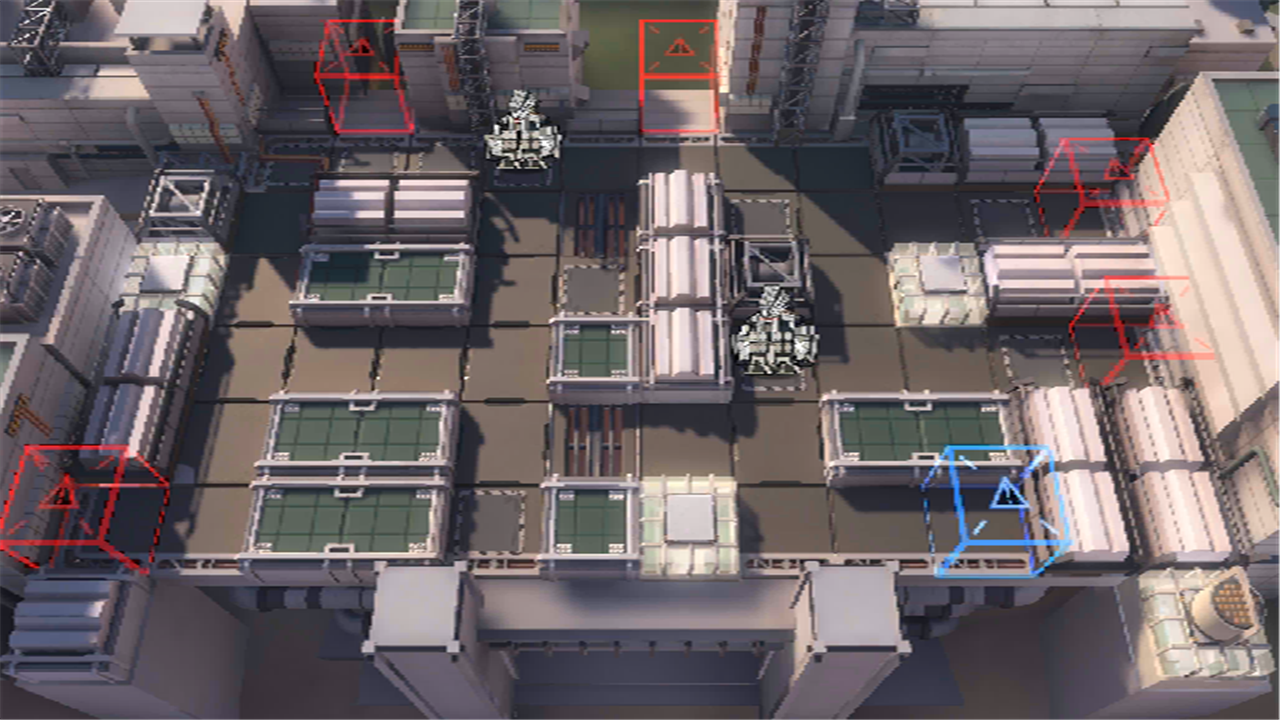
\includegraphics[scale=0.685,angle=270]{other/map.png}}

\end{document}
